% SPDX-License-Identifier: CC-BY-SA-4.0
% Author: Matthieu Perrin
% Part: 
% Section: 
% Sub-section: 
% Frame: 

\begingroup

\SetKwFunction{Lock}{lock}
\SetKwFunction{Unlock}{unlock}

\newcommand\Frenchie[3]{
  \begin{tikzpicture}
    \draw      (0,0)     node{\includegraphics[height=2.5cm]{#2}};
    \draw[#3]  (-.1,-.3) node{\Large #1};
  \end{tikzpicture}
}

\newcommand\FrenchieStructure[1]{\Frenchie{#1}{frenchieBleu} {structure}}
\newcommand\FrenchieAlert[1]    {\Frenchie{#1}{frenchieRouge}{alert}}
\newcommand\FrenchieExample[1]  {\Frenchie{#1}{frenchieVert} {example}}
\newcommand\FrenchieRight[1]    {\Frenchie{#1}{frenchieDroit}{structure}}

\begin{frame}[fragile]{Algorithme simplifié}

  \on[text,top]{
    \begin{algorithm}[H]
      \SVariables{}{
        \Structure<2>{$tickets[n] \leftarrow [\infty, ..., \infty]$}\;
      }
      ~\\
      \Operation{$\Lock()$}{
        \nl \Example<6>{\Structure<3>{$tickets[i] \leftarrow 0$}}\;
        \nl \Structure<4>{\Let $t_i$ \St $\displaystyle \left\langle t_i,i \right\rangle > \max_{j : tickets[j] < \infty} \Alert<6>{\left\langle tickets[j], j\right\rangle}$}\;
        \nl \Alert<6>{\Structure<4>{$tickets[i] \leftarrow t_i$}}\;
        \nl \Structure<5>{\Wait $\displaystyle \left\langle t_i,i \right\rangle = \min_j \Example<6>{\left\langle tickets[j], j \right\rangle}$}.
      }
      ~\\
      \Operation{$\Unlock()$}{
        \Structure<2>{$tickets[i] \leftarrow \infty$}.
      }
    \end{algorithm}
  }

  \onBlock<6>[bottom]{Exclusion mutuelle:}{
    Supposons $p_i$ et $p_j$ en section critique, avec $\left\langle t_i,i \right\rangle < \left\langle t_j,j \right\rangle$

    \vspace{3mm}
    \begin{tikzpicture}[y=7mm, anchor=mid]
      \draw[->] (0,0) node[left]{$p_i$} -- (6,0) ;
      \draw[->] (0,1) node[left]{$p_j$} -- (6,1) ;

      \footnotesize
      \node[operation, example, fill=example!20] at (1.5,1) {1: $tickets[i] \leftarrow 0$};
      \node[operation, alert, fill=alert!20]     at (4  ,1) {2: $tickets[j] \rightarrow {<t_j}$};
      \node[operation, alert, fill=alert!20]     at (1.5,0) {3: $tickets[j] \leftarrow t_j$};
      \node[operation, example, fill=example!20] at (4  ,0) {4: $tickets[i] \rightarrow \infty$};
    \end{tikzpicture}
  }
  
  \ob<2>  [x= 35mm,y= 10mm]{\FrenchieStructure{$\infty$}}
  \ob<4>  [x=-50mm,y=-30mm]{\FrenchieRight{$3$}}
  \ob<2-4>[x=-28mm,y=-30mm]{\FrenchieAlert{$2$}}
  \ob<2-4>[x=-06mm,y=-30mm]{\FrenchieExample{$1$}}
  \ob<3>  [x= 16mm,y=-30mm]{\FrenchieStructure{$0$}}
  \ob<5>  [x= 16mm,y=-30mm]{\FrenchieRight{$3$}}
  \ob     [x= 45mm,y=-30mm]{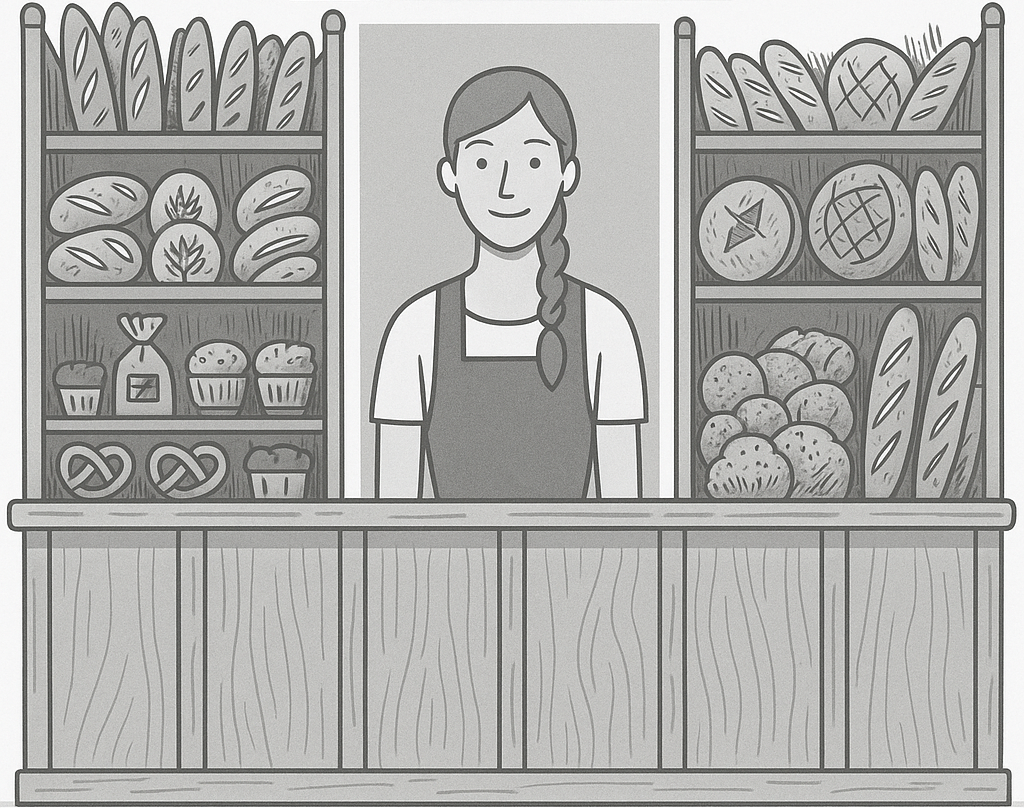
\includegraphics[height=3.3cm]{bakery}}
  
\end{frame}

\endgroup
\endinput
